\newpage
\section{Resultater}
For at brugeren kan følge sin egen udvikling er der implementeret et BarChart. Denne graf viser tiden, brugeren har trænet for den givne uge. Af denne graf plottes en træningstid for hver af ugens dage. Af \autoref{fig:koderesul} fremgår et udpluk af implementeringen for den opstillede graf.

\begin{figure} [H]
\centering
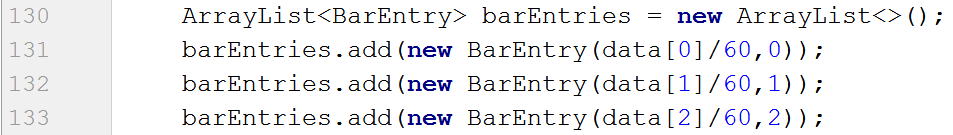
\includegraphics[width=0.9\textwidth]{figures/imple/koderesul}
\caption{Udklip af javakode for BarChart, der senere har til formål at illustrere brugerens ugentlige træningstid.}
\label{fig:koderesul}
\end{figure} 

\noindent
Der ses af dette udklip, at der oprettes et ArrayList under navnet \textit{barEntries}. Dette array anvendes til at lagre mængden af data, der ønskes plottet. Dertil ses det, hvorledes nye elementer tilføjes dette array ud fra en værdi og index. Værdien, der instættes tages fra et andet array af navnet \textit{data}, hvori der lagres en træningstid for ugens dage. Plads nummer \textit{0} refererer til den første dag i ugen og tæller således op efter ugens dage. \textit{Data} er divideret med 60, da træningstiden er gemt som sekunder og ønskes plottet i minutter. 

Belønninger gives udfra samlet tid, afstand, antal træninger samt antal konditionstræninger og beregnes efter endt træning. Da disse belønninger er baseret ud fra den samlede træning, hentes den sammenlagte tid, afstand samt totale antal træninger fra databasen og omregnes til et tal mellem 1 til 6, der repræsenterer antallet af stjerner brugeren har opnået. Et udklip af javakoden for omregningen for brugere med en kategorisering \textit{A} ses af \autoref{fig:kodebelon}.

\begin{figure} [H]
\centering
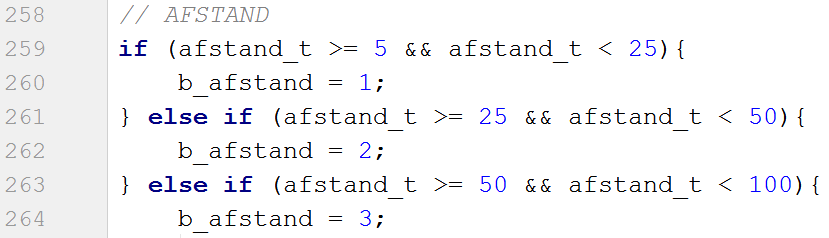
\includegraphics[width=0.7\textwidth]{figures/imple/kodebelon}
\caption{Udklip af javakode for omregning af samlet afstand til optjente belønninger for brugere med kategorisering \textit{A}.}
\label{fig:kodebelon}
\end{figure} 

\noindent
Det fremgår af dette javaudklip, at omregningen foregår ved if/else-loops. Hvis afstanden ligger indenfor et interval af 5 og 25, sættes \textit{b\_afstand} lig 1, hvilket repræsenterer én stjerne. Af \autoref{tab:SamletBelon} fremgår kriterierne for at opnå stjerner for brugere med kategoriseringen \textit{A}.  

\begin{table}[H]
\centering
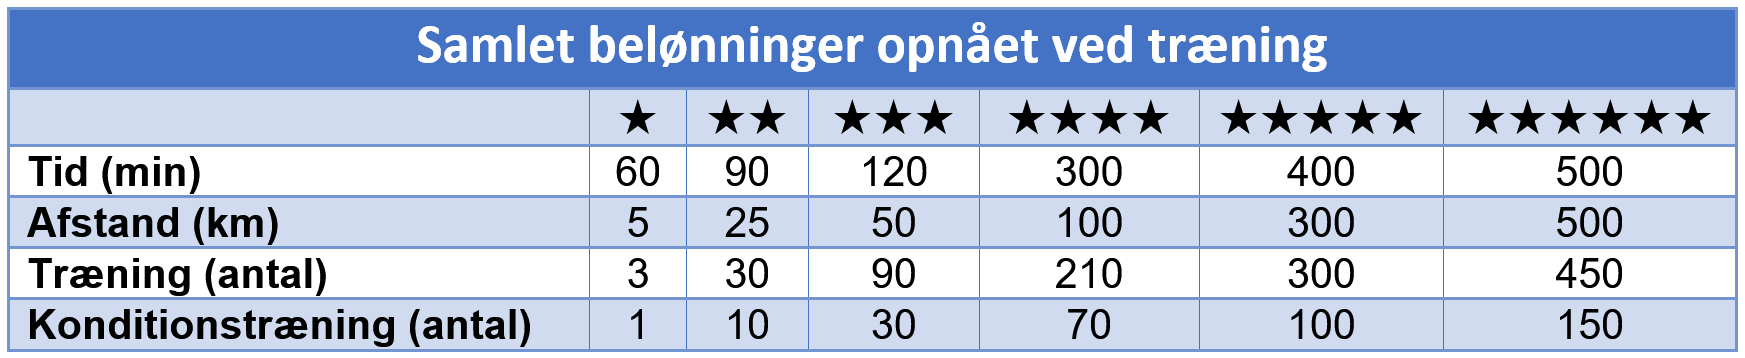
\includegraphics[width=1\textwidth]{figures/imple/SamletBelon}
\caption{Kriterier for at opnå belønninger inden for henholdsvis samlet tid, afstand og total antal træninger samt konditionstræninger for brugere med kategorisering \textit{A}.}
\label{tab:SamletBelon}
\end{table}  
